
\item Two ideal batteries of emf \(V_1\) and \(V_2\) and three resistances \(R_1\), \(R_2\) and \(R_3\) are connected as shown in the figure. The current in resistance \(R_2\) would be zero if
    \begin{center}
        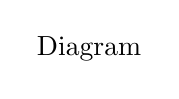
\begin{tikzpicture}
            % Since the actual circuit diagram cannot be recreated using LaTeX code without a full description,
            % a placeholder for the diagram is placed here. 
            \node at (0, 0) {Diagram};
        \end{tikzpicture}
    \end{center}
    \begin{tasks}(2)
        \task \(V_1 = V_2\) and \(R_1 = R_2 = R_3\)
        \task \(V_1 = V_2\) and \(R_1 = 2R_2 = R_3\)
        \task \(V_1 = 2V_2\) and \(2R_1 = 2R_2 = R_3\)
        \task \(2V_1 = V_2\) and \(2R_1 = R_2 = R_3\)
    \end{tasks}
